\documentclass[11pt]{article}
\usepackage[english]{babel}
\usepackage[numbers]{natbib} 
\usepackage{url}
\usepackage[utf8]{inputenc}
\usepackage{amsmath}
\usepackage{amssymb}
\usepackage{graphicx}
\usepackage{parskip}
\usepackage{fancyhdr}
\usepackage{vmargin}
\usepackage{booktabs}
\usepackage[table,xcdraw]{xcolor}
\usepackage{tabularx}
\usepackage{caption} 
\usepackage{float}
\usepackage{longtable}
\usepackage{array}
\usepackage{caption}
\usepackage{subcaption}

\usepackage[colorlinks = true,
linkcolor = black,
urlcolor  = black,
citecolor = black,
anchorcolor = black]{hyperref}

\setmarginsrb{3 cm}{1 cm}{3 cm}{1 cm}{1 cm}{1.5 cm}{1 cm}{1.5 cm}

\newcolumntype{L}[1]{>{\raggedright\let\newline\\\arraybackslash\hspace{0pt}}m{#1}}
\newcolumntype{C}[1]{>{\centering\let\newline\\\arraybackslash\hspace{0pt}}m{#1}}
\newcolumntype{R}[1]{>{\raggedleft\let\newline\\\arraybackslash\hspace{0pt}}m{#1}}

\title{Assignment \#3 - Protein Classification}
\date{\today}

\makeatletter
\let\thetitle\@title
\let\thesubtitle\@subtitle
\let\theauthor\@author
\let\thedate\@date
\makeatother

\pagestyle{plain}

\captionsetup[table]{skip=5pt}

\makeatletter
\renewcommand*\l@section{\@dottedtocline{1}{1.5em}{2.3em}}
\makeatother


\begin{document}
	
%%%%%%%%%%%%%%%%%%%%%%%%%%%%%%%%%%%%%%%%%%%%%%%%%%%%%%%%%%%%%%%%%%%%%%%%%%%%%%%%%%%%%%%%%

\begin{titlepage}
	\centering
	\textsc{\LARGE University of Coimbra}\\[1.0 cm]
	\textsc{\large Doctoral Program in Information Science and Technology}\\[0.5 cm]
	\textsc{\large Real Time Learning in Intelligent Systems}\\[5 cm]
	\rule{\linewidth}{0.2 mm} \\[0.4 cm]
	{ \LARGE \bfseries \thetitle}\\ [0.2 cm]
	\rule{\linewidth}{0.2 mm} \\[3 cm]
	
	\textsc{Joaquim Pedro Bento Gonçalves Pratas Leitão - 2011150072}\\[5 cm]
	
	{\large \thedate}\\[2 cm]
	
	\vfill
	
\end{titlepage}

\tableofcontents

\newpage

%%%%%%%%%%%%%%%%%%%%%%%%%%%%%%%%%%%%%%%%%%%%%%%%%%%%%%%%%%%%%%%%%%%%%%%%%%%%%%%%%%%%%%%%%

\section{Introduction}
\label{introduction}

The protein classification problem is among the most important and fundamental problems in computational biology. In short, this problem can be defined as the task of classifying proteins into functional and structural classes based on \emph{homology} (evolutionary similarity) of protein sequence data.

Several approaches can be taken to solve the protein classification problem, ranging from methods that analyse the protein's coding sequence in the genetic code, to more complex approaches that study the 3D structure of the proteins in order to perform such classification.

In the current assignment, a sequence similarity-based approach to this problem will be adopted. The algorithms and methods to be applied fall in the first set of practices mentioned in the previous paragraph. As such, the current work will focus on analysing the genetic sequence responsible for coding a given protein. Browsing solutions for this problem proposed in the literature Support Vector Machines appear as interesting techniques, achieving promising results \cite{leslie2002mismatch, zavaljevski2002support, cai2003svm}.

\subsection{Objectives}

One major high-level objective can be identified in the present assignment: For any given protein determine its functional class by analysing its coding sequence.

This work will feature data from the \emph{SCOP Database}\cite{murzin1995scop}, more precisely the \emph{SCOP40} dataset\footnote{\url{http://pongor.itk.ppke.hu/benchmark}}. This dataset contains genetic sequences responsible for coding proteins of 55 different families. Therefore, a more low-level objective for this work is to develop classifiers capable of identifying protein sequences belonging in each of the 55 families.

The current assignment also featured a secondary objective, consisting in comparing incremental with non-incremental classifier approaches. 

\subsection{Methodology}
\label{methodology}

In light of the description of the assignment at hand, and its objectives, the following steps will be considered in the work to be performed:

\begin{enumerate}
	\item Initial dataset preprocessing
	
	\item Data representation
	
	\item Classifier training
	
	\item Results assessment
\end{enumerate}

In an initial stage, a preprocessing of the \emph{SCOP40} data was conducted, aiming to construct a training and testing dataset for each one of the 55 families in the dataset. It is worth mentioning that even though the \emph{SCOP Database} does not provide separate training and testing datasets for each family, it proposes a list of instances to be used for training and testing, for each family. Therefore, at this stage, the preprocessing step consisted in analysing the provided mapping and in creating individual train and test files for each family.

Probably the most important step in this assignment, data representation can be seen as an advanced preprocessing step to transform the data to be feed to a classifier. It strongly conditions the final performance of the classifiers as an inappropriate representation does not allow for a good separation of the data, therefore leading to poor classification performance. In this work the \emph{segmentation} was the representation technique implemented. Section \ref{data_representation} covers this technique in detail.

Following the representation classifiers needed to be properly trained and tested. In this work \emph{incremental} and \emph{non-incremental} classifiers were intended to be compared. In this sense two different but somewhat related classifiers were selected: \emph{LASVM}, as the incremental classifier; and \emph{Support Vector Machines (SVM)}, as the non-incremental classifier.

As each protein sequence under analysis must be assigned to one of 55 possible families, a multi-class classification problem is being considered. In this sense one classifier for each family must be develop. Considering that two different classifiers are intended to be compared, two classifiers were trained for each family (one \emph{LASVM} and one \emph{SVM}).

Finally, once the classifiers were properly created and trained, their performance was assessed with the testing dataset, following an analysis of the test results in order to determine which approach registered better results, if any. Considering the fact that the \emph{SCOP40} is an highly unbalanced dataset (indeed, a fact that is very common in problems of this nature in computational biology) the different approaches were not compared with respect to their accuracy, but with respect to the \emph{Area Under Curve} (AUC) metric.

Concerning the classifiers' development and all \emph{assignment-related} tasks, the \emph{R}\footnote{\url{https://www.r-project.org/}} software environment was selected as the implementation and working tool.

\subsection{Document Outline}

The remainder of this document is organised as follows: Section \ref{dataset_description} introduces and describes the dataset used in the current work. Section \ref{data_representation} addresses the data representation technique adopted in this assignment. Sections \ref{svm} and \ref{lasvm} cover the experimental results obtained with the two techniques being compared in this work. Finally, section \ref{conclusions} presents a reflective analysis of the obtained experimental results and identifies directions to be explored in future work.


\section{Dataset Description}
\label{dataset_description}

The \emph{SCOP40} dataset contains information concerning the genetic coding sequences of different proteins and their corresponding families, being organised in two main files, as follows:

\begin{itemize}
	\item \emph{SCOP40mini.fasta} - Text file listing the different genetic coding sequences for several proteins. A unique identifier is also presented for each protein sequence.
	
	\item \emph{SCOP40mini\_sequence\_minidatabase\_19.cast} - Text file containing a mapping between each family and the protein sequences of the \emph{SCOP40mini.fasta} file to be used during classifier training or test.
\end{itemize}

\section{Data Representation}
\label{data_representation}

Referenced in section \ref{methodology}, the representation technique implemented in the current work was the \emph{segmentation} method. In short, this method consists in, for each protein sequence, count the number of occurrences of each individual nucleotide (that is, of each letter in the sequence).

For example, consider the following example protein sequence: \emph{"vdaeavvqqkcis"}. The segmentation method would output a total number of 3 occurrences for the \emph{"v"} nucleotide, 1 occurrence for the \emph{"d"} nucleotide, and so on. The only exception is for \emph{"x"} nucleotides, which represent missing information about a nucleotide in the protein sequence, and therefore are discarded in this exercise. Figure \ref{representation_example} presents an example of the output of this method for a protein sequence. 

\begin{figure}[h]
	\centering
	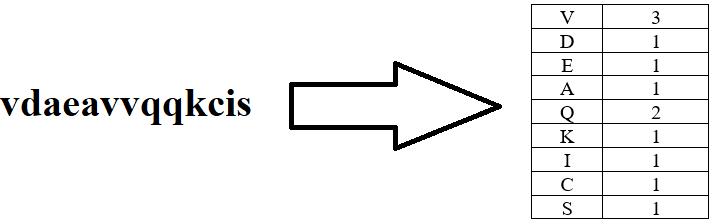
\includegraphics[scale=0.7]{images/representation.png}
	\caption{Example of the implemented segmentation representation for a protein sequence.}
	\label{representation_example}
\end{figure}

As it is not mandatory that each protein sequence contains all possible individual nucleotides, this method requires an initial passage for all the sequences in the dataset, in order to identify all individual nucleotides. The method's output will, therefore, present the number of occurrences of each of those nucleotides in the current protein sequence being analysed.

\section{Support Vector Machines}
\label{svm}

\emph{Support Vector Machines} (SVM) \cite{cortes1995support} are supervised machine learning algorithms applied in classification and regression tasks. During SVM training a model is built using a set of labelled samples (which can belong to one of two possible classes). Such model can then be used to classify new samples, that is, assign a new sample to a previously defined and learned class.

During training an hyperplane that assures the largest separation between instances of both classes is sought. The data points that lie closest to the hyperplane are called \emph{support vectors} and determine the separation margin between the two classes. Because of their (usually) small distance to the separation hyperplane these are the most difficult data points to classify. Misclassification of some instances may or may not be allowed. Such behaviour is controlled by a \emph{cost} parameter $C$ that penalises misclassification.

Even though SVMs seek a linear hyperplane, and therefore perform a linear classification task, they have also been extensively applied in non-linear classification problems. When performing non-linear classification, SVMs need to map the samples into a higher dimensional space, where a linear separation hyperplane can be computed. Once such a hyperplane has been determined an inverse transformation can be performed, mapping the data back to the original space. Such mapping operation is defined as a \emph{kernel}. For this reason, and since most \emph{application} problems are non-linear, SVMs are considered \emph{kernel methods}.

Several high-dimensional mappings, or \emph{kernels}, have been proposed in the literature for SVMs, though typical kernels covered in SVM books include: \emph{linear}, \emph{polynomial}, \emph{sigmoid} and \emph{radial basis function} (RBF).

In the current work, SVMs featuring a RBF kernel are intended to be applied. RBF kernels are defined by the following mathematical expression: $exp(- \gamma * |x_{i}-x_{j}|^2) $. Therefore, SVM training and classification performance will be influenced by the values defined for the cost and RBF parameters: $C$ and $\gamma$, respectively.

Considering that no prior knowledge of adequate values for these parameters has been obtained, optimal values must be searched. As suggested by Hsu \emph{et al.} \cite{hsu2003practical}, a good practice to tune these parameters is to perform a grid search with exponentially growing sequences of $C$ and $\gamma$ (for example $C \: = \: 2^{-5}, 2^{-4}, \cdots , 2^{5}$ and $\gamma \: = \: 2^{-15}, 2^{-14}, \cdots , 2^{3}$).

As mentioned in section \ref{methodology}, all algorithms used throughout the work were implemented in the \emph{R} software environment. With respect to SVMs, the \emph{e1071}\footnote{\url{https://CRAN.R-project.org/package=e1071}} package was used, providing an interface in the R programming language for the popular SVM library, \emph{LIBSVM} \cite{CC01a}.

Supported by the suggestion of Hsu \emph{et al.}, a grid search method was adopted to tune the SVM parameters in this task. As 55 different classifiers are intended to be trained (one for each family), the mentioned tuning process was repeated for each of the 55 trained classifiers. In this grid search exercise, the following ranges of values were defined:

\begin{itemize}
	\item For the cost parameter, $C$, the defined ranged included values from $10^{-3}$ up to $10^{3}$ in a logarithmic scale: $10^{-3}, 10^{-2}, \cdots , 10^{3}$
	
	\item For the kernel parameter, $\gamma$, the defined range included values from $10^{-4}$ up to $10^{4}$, also in a logarithmic scale: $10^{-4}, 10^{-3}, \cdots , 10^{4}$
\end{itemize}

For each combination of values $(C, \gamma)$ - and for each family - a classifier was trained and its performance was registered in both the training and test dataset, using the \emph{AUC} metric. The combination of parameters that produced the best results (higher AUC in the test dataset) for each family are presented in Table \ref{svm_results}.

An average AUC of $0.74$ in the test dataset was recorded. The best results in the test dataset were recorded in family \emph{"SCOP40\_b.29.1.\_b.29.1.2."}, with an AUC of $0.99$ and an SVM with the following parameters: $C = 256$ and $\gamma = 3.9e-03$. It is also worth pointing out that, for this classifier a cost of $256$ was defined. Even though much higher cost values can be found in Table \ref{svm_results}, this still remains an high cost value, suggesting a \emph{hard-limit} SVM.

Unfortunately, for some families worse results were registered: In the cases of families \emph{"SCOP40\_b.29.1.\_b.29.1.3."}, \emph{"SCOP40\_c.23.16.\_c.23.16.2."}, \emph{"SCOP40\_c.3.1.\_c.3.1.5."},\\\emph{"SCOP40\_c.68.1.\_c.68.1.13."} and \emph{"SCOP40\_d.81.1.\_d.81.1.3."} the best AUC in both the train and test dataset was $0.5$; while in the cases of families \emph{"SCOP40\_c.26.2.\_c.26.2.1."} and \emph{"SCOP40\_c.47.1.\_c.47.1.10."} clear overfitting scenarios can be identified, as to a train AUC of 1 corresponded a test AUC of about $0.5$.

\begin{longtable}{|p{.33\textwidth}|p{.1\textwidth}|p{.13\textwidth}|p{.15\textwidth}|p{.15\textwidth}|}
	\hline
	\textbf{Family}               & \textbf{Cost} & \textbf{Gamma}   & \textbf{AUC Train} & \textbf{AUC Test} \\ \hline
	SCOP40\_a.118.1.\_a.118.1.14. & 8192  & 1.95e-03  & 0.90  & 0.82  \\ \hline
	
	SCOP40\_a.3.1.\_a.3.1.1.      & 16384 & 4.8e-04   & 0.83  & 0.76  \\ \hline
	
	SCOP40\_a.39.1.\_a.39.1.2.    & 32    & 7.8e-03   & 0.80  & 0.75  \\ \hline
	
	SCOP40\_a.39.1.\_a.39.1.5.    & 32768 & 3.05e-05  & 0.69  & 0.83  \\ \hline
	
	SCOP40\_a.4.1.\_a.4.1.1.      & 1     & 0.125     & 0.73  & 0.87  \\ \hline
	
	SCOP40\_a.4.1.\_a.4.1.3.      & 1     & 1         & 0.97  & 0.90  \\ \hline
	
	SCOP40\_a.4.1.\_a.4.1.9.      & 128   & 0.125     & 1     & 0.71  \\ \hline
	
	SCOP40\_a.4.5.\_a.4.5.28.     & 16    & 0.125     & 0.96  & 0.91  \\ \hline
	
	SCOP40\_b.1.1.\_b.1.1.2.      & 1     & 0.125     & 0.93  & 0.98  \\ \hline
	
	SCOP40\_b.1.1.\_b.1.1.3.      & 16    & 0.25      & 1     & 0.92  \\ \hline
	
	SCOP40\_b.1.1.\_b.1.1.4.      & 32    & 0.0625    & 0.98  & 0.82  \\ \hline
	
	SCOP40\_b.1.18.\_b.1.18.2.    & 64    & 0.0625    & 0.97  & 0.74  \\ \hline
	
	SCOP40\_b.29.1.\_b.29.1.11.   & 8     & 0.0156    & 0.72  & 0.90  \\ \hline
	
	SCOP40\_b.29.1.\_b.29.1.2.    & 256   & 3.9e-03   & 0.77  & 0.99  \\ \hline
	
	SCOP40\_b.29.1.\_b.29.1.3.    & 0.031 & 3.05e-05 & 0.5    & 0.5   \\ \hline
	
	SCOP40\_b.29.1.\_b.29.1.4.    & 2     & 0.25     & 0.99   & 0.57  \\ \hline
	
	SCOP40\_b.40.4.\_b.40.4.3.    & 512   & 0.031    & 0.99   & 0.63  \\ \hline
	
	SCOP40\_b.40.4.\_b.40.4.4.    & 4     & 0.125    & 0.82   & 0.69  \\ \hline
	
	SCOP40\_b.40.4.\_b.40.4.5.    & 1024  & 0.031    & 1      & 0.70  \\ \hline
	
	SCOP40\_b.40.4.\_b.40.4.6.    & 4     & 0.125    & 0.86   & 0.70  \\ \hline
	
	SCOP40\_b.47.1.\_b.47.1.1.    & 4     & 0.125    & 1      & 0.65  \\ \hline
	
	SCOP40\_b.6.1.\_b.6.1.1.      & 1     & 0.125    & 0.72   & 0.55  \\ \hline
	
	SCOP40\_b.6.1.\_b.6.1.3.      & 4096  & 9.8e-04  & 0.78   & 0.63  \\ \hline
	
	SCOP40\_c.1.8.\_c.1.8.3.      & 8192  & 3.05e-05 & 0.88   & 0.88  \\ \hline
	
	SCOP40\_c.1.8.\_c.1.8.5.      & 256   & 1.95e-03 & 0.94   & 0.76  \\ \hline
	
	SCOP40\_c.10.2.\_c.10.2.5.    & 0.031 & 3.05e-05 & 0.5    & 0.5   \\ \hline
	
	SCOP40\_c.2.1.\_c.2.1.2.      & 4096  & 9.8e-04  & 0.83   & 0.76  \\ \hline
	
	SCOP40\_c.2.1.\_c.2.1.3.      & 32    & 0.0625   & 1.00   & 0.67  \\ \hline
	
	SCOP40\_c.2.1.\_c.2.1.4.      & 16    & 0.0625   & 0.98   & 0.86  \\ \hline
	
	SCOP40\_c.2.1.\_c.2.1.5.      & 8     & 0.125    & 0.99   & 0.80  \\ \hline
	
	SCOP40\_c.2.1.\_c.2.1.6.      & 4     & 0.125    & 0.97   & 0.78  \\ \hline
	
	SCOP40\_c.2.1.\_c.2.1.7.      & 16    & 0.031    & 0.91   & 0.81  \\ \hline
	
	SCOP40\_c.23.16.\_c.23.16.2.  & 0.031 & 3.05e-05 & 0.5    & 0.5   \\ \hline
	
	SCOP40\_c.26.2.\_c.26.2.1.    & 32    & 0.031    & 1      & 0.56  \\ \hline
	
	SCOP40\_c.3.1.\_c.3.1.4.      & 128   & 0.016    & 0.82   & 0.58  \\ \hline
	
	SCOP40\_c.3.1.\_c.3.1.5.      & 0.031 & 3.05e-05 & 0.5    & 0.5   \\ \hline
	
	SCOP40\_c.37.1.\_c.37.1.10.   & 32768 & 9.8e-04  & 0.95   & 0.78  \\ \hline
	
	SCOP40\_c.37.1.\_c.37.1.11.   & 8     & 0.031    & 0.92   & 0.88  \\ \hline
	
	SCOP40\_c.37.1.\_c.37.1.12.   & 8     & 0.125    & 0.99   & 0.89  \\ \hline
	
	SCOP40\_c.37.1.\_c.37.1.19.   & 1024  & 2.4e-04  & 0.77   & 0.82  \\ \hline
	
	SCOP40\_c.37.1.\_c.37.1.20.   & 32768 & 1.9e-03  & 0.97   & 0.87  \\ \hline
	
	SCOP40\_c.37.1.\_c.37.1.5.    & 2     & 0.0625   & 0.91   & 0.67  \\ \hline
	
	SCOP40\_c.37.1.\_c.37.1.6.    & 128   & 1.9e-03  & 0.81   & 0.95  \\ \hline
	
	SCOP40\_c.37.1.\_c.37.1.8.    & 64    & 0.0625   & 1      & 0.79  \\ \hline
	
	SCOP40\_c.37.1.\_c.37.1.9.    & 1024  & 3.05e-05 & 0.67   & 0.83  \\ \hline
	
	SCOP40\_c.47.1.\_c.47.1.1.    & 32    & 0.0625   & 0.90   & 0.71  \\ \hline
	
	SCOP40\_c.47.1.\_c.47.1.10.   & 16    & 0.25     & 1      & 0.56  \\ \hline
	
	SCOP40\_c.47.1.\_c.47.1.2.    & 512   & 0.0625   & 1      & 0.72  \\ \hline
	
	SCOP40\_c.47.1.\_c.47.1.5.    & 32    & 0.0625   & 0.93   & 0.55  \\ \hline
	
	SCOP40\_c.55.1.\_c.55.1.1.    & 128   & 0.031    & 1      & 0.67  \\ \hline
	
	SCOP40\_c.67.1.\_c.67.1.3.    & 2     & 0.0625   & 1      & 0.87  \\ \hline
	
	SCOP40\_c.67.1.\_c.67.1.4.    & 2     & 0.0312   & 0.97   & 0.96  \\ \hline
	
	SCOP40\_c.68.1.\_c.68.1.13.   & 0.031 & 3.05e-05 & 0.5    & 0.5   \\ \hline
	
	SCOP40\_d.81.1.\_d.81.1.3.    & 0.031 & 3.05e-05 & 0.5    & 0.5   \\ \hline
	
	SCOP40\_e.8.1.\_e.8.1.1.      & 2     & 0.031    & 0.83   & 0.6   \\ \hline
	\caption{SVM configurations that produced the best results in the training dataset.}
	\label{svm_results}
\end{longtable}

\section{LASVM}
\label{lasvm}

The application of Support Vector Machines (and other similar approaches) in real-life problems is strongly restricted by their dimensionality and scale. Indeed, when training examples are abundant and of high dimensionality the computational and time resources needed to train these approaches are significant.

In response to such limitations incremental approaches have been proposed in the literature which, while analysing each sample individually, do not give equal attention to all of the training data. In the field of SVMs incremental techniques repeatedly train a model with a smaller training subset, keeping only the support vectors between training iterations.

In the scope of this work, the incremental alternative to SVMs intended to be studied is the \emph{LASVM}. In their proposal of the algorithm, Bordes \emph{et al.} \cite{bordes-ertekin-weston-bottou-2005} provided two ways of defining this algorithm: On one hand LASVM can be defined as an online version of the SVM featuring a support vector removal step; another possible view of this algorithm is related with its reorganization of the SMO sequential direction searches. More detailed information concerning this algorithm and its properties can be found in the cited literature.

The authors of \cite{bordes-ertekin-weston-bottou-2005} also provided a complete implementation of their proposed algorithm\footnote{\url{http://leon.bottou.org/projects/lasvm}}. Similarly to the \emph{SVM} case, an \emph{R} package providing an interface to the \emph{LASVM} algorithm implementation was used: \emph{lasvmR}\footnote{\url{https://CRAN.R-project.org/package=lasvmR}}.

Similarly to the approach presented in the previous section, and followed in the development of the non-incremental SVM classifiers, a grid search method was adopted to tune the parameters of the LASVM classifiers. As the LASVM is an online version of the SVM it features the same parameters as the SVM, with the same meaning.

In this sense, the ranges defined in section \ref{svm} were also considered at this point. Additionally, the performance of the trained LASVM classifiers in both the train and test datasets was also registered, with the parameters' combinations that produced the best results (in terms of AUC in the test dataset) for each family are presented in Table \ref{lasvm_results}.

Overall, classifications performed with the \emph{LASVM} produce more accurate results, supported by higher test AUC values for the majority of the families. In some families where it was not possible to learn a classifier with the SVM method, the LASVM allows for more accurate results: this is the case for the families \emph{"SCOP40\_b.29.1.\_b.29.1.3."}, \emph{"SCOP40\_c.23.16.\_c.23.16.2."}, \emph{"SCOP40\_c.3.1.\_c.3.1.5."} and \emph{"SCOP40\_c.68.1.\_c.68.1.13."}.

An average AUC of $0.81$ in the test dataset was recorded using the LASVM. The best results in the test dataset were recorded in families \emph{"SCOP40\_b.29.1.\_b.29.1.11."},\\ \emph{"SCOP40\_b.29.1.\_b.29.1.2."} and \emph{"SCOP40\_c.67.1.\_c.67.1.4."} where an AUC of $0.99$ was registered. The parameters of the LASVM classifiers in these cases were: $C = 32$ and $\gamma = 1.22e-04$ for the first family; $C = 4$ and $\gamma = 9.7e-04$ for the second family; and $C = 512$ and $\gamma = 2.44e-04$ for the third family.

With the exception of the third family, it can be seen that the cost parameter is clearly smaller in the LASVM case, yielding a \emph{soft-limit} classifier (or at least less \emph{hard-limit} than the SVM alternative).

Like in the previous exercise, in some cases it was not possible to learn a classifier, resulting in an AUC of around $0.5$ in both the train and test datasets. This was the case for families \emph{"SCOP40\_c.10.2.\_c.10.2.5."} and \emph{"SCOP40\_d.81.1.\_d.81.1.3."}. Unlike with the SVM classifiers, the LASVM does not appear to be suffering of overfitting in any situation: indeed, whenever a high AUC in the training was registered an also higher AUC was registered in the test dataset.

\begin{longtable}{|p{.33\textwidth}|p{.1\textwidth}|p{.13\textwidth}|p{.15\textwidth}|p{.15\textwidth}|}
	\hline
	\textbf{Family}               & \textbf{Cost} & \textbf{Gamma}   & \textbf{AUC Train} & \textbf{AUC Test} \\ \hline
	SCOP40\_a.118.1.\_a.118.1.14. & 256     & 2.44e-04   & 0.97 & 0.91 \\ \hline

	SCOP40\_a.3.1.\_a.3.1.1.      & 8192    & 2.44e-04   & 0.93 & 0.87 \\ \hline

	SCOP40\_a.39.1.\_a.39.1.2.    & 512     & 6.10e-05   & 0.87 & 0.81 \\ \hline

	SCOP40\_a.39.1.\_a.39.1.5.    & 1024    & 3.05e-05   & 0.76 & 0.90 \\ \hline

	SCOP40\_a.4.1.\_a.4.1.1.      & 16      & 9.7e-04    & 0.88 & 0.95 \\ \hline

	SCOP40\_a.4.1.\_a.4.1.3.      & 0.25    & 3.9e-03    & 0.76 & 0.90 \\ \hline
	
	SCOP40\_a.4.1.\_a.4.1.9.      & 8192    & 4.8e-04    & 0.98 & 0.86 \\ \hline
	
	SCOP40\_a.4.5.\_a.4.5.28.     & 64      & 2.4e-04    & 0.77 & 0.92 \\ \hline
	
	SCOP40\_b.1.1.\_b.1.1.2.      & 4       & 9.8e-04    & 0.92 & 0.98 \\ \hline
	
	SCOP40\_b.1.1.\_b.1.1.3.      & 32      & 3.9e-03    & 1    & 0.92 \\ \hline
	
	SCOP40\_b.1.1.\_b.1.1.4.      & 32768   & 1.2e-04    & 0.94 & 0.86 \\ \hline
	
	SCOP40\_b.1.18.\_b.1.18.2.    & 4096    & 9.8e-04    & 0.99 & 0.72 \\ \hline
	
	SCOP40\_b.29.1.\_b.29.1.11.   & 32      & 1.22e-04   & 0.74 & 0.99 \\ \hline
	
	SCOP40\_b.29.1.\_b.29.1.2.    & 4       & 9.7e-04    & 0.78 & 0.99 \\ \hline
	
	SCOP40\_b.29.1.\_b.29.1.3.    & 4096    & 1.22e-04   & 0.80  & 0.69 \\ \hline
	
	SCOP40\_b.29.1.\_b.29.1.4.    & 8192    & 1.22e-04   & 0.89  & 0.81 \\ \hline
	
	SCOP40\_b.40.4.\_b.40.4.3.    & 32768   & 1.22e-04   & 0.81  & 0.73 \\ \hline
	
	SCOP40\_b.40.4.\_b.40.4.4.    & 32768   & 4.88e-04  & 0.89  & 0.89 \\ \hline
	
	SCOP40\_b.40.4.\_b.40.4.5.    & 8192    & 4.88e-04  & 0.99  & 0.82 \\ \hline
	
	SCOP40\_b.40.4.\_b.40.4.6.    & 8192    & 9.76e-04  & 0.99  & 0.73 \\ \hline
	
	SCOP40\_b.47.1.\_b.47.1.1.    & 8192    & 6.10e-05  & 0.95  & 0.73 \\ \hline
	
	SCOP40\_b.6.1.\_b.6.1.1.      & 8192    & 6.10e-05  & 0.70  & 0.73 \\ \hline
	
	SCOP40\_b.6.1.\_b.6.1.3.      & 128     & 4.88e-04  & 0.94  & 0.64 \\ \hline
	
	SCOP40\_c.1.8.\_c.1.8.3.      & 4096    & 6.10e-05  & 0.96  & 0.93 \\ \hline
	
	SCOP40\_c.1.8.\_c.1.8.5.      & 8192    & 1.22e-04  & 0.99  & 0.84 \\ \hline
	
	SCOP40\_c.10.2.\_c.10.2.5.    & 0.03125 & 3.05e-05  & 0.5   & 0.5  \\ \hline
	
	SCOP40\_c.2.1.\_c.2.1.2.      & 4096    & 1.22e-04  & 0.96  & 0.73 \\ \hline
	
	SCOP40\_c.2.1.\_c.2.1.3.      & 2048    & 1.22e-04  & 0.89  & 0.76 \\ \hline
	
	SCOP40\_c.2.1.\_c.2.1.4.      & 128     & 2.44e-04  & 0.89  & 0.91 \\ \hline
	
	SCOP40\_c.2.1.\_c.2.1.5.      & 0.5     & 2.44e-04  & 0.82  & 0.86 \\ \hline
	
	SCOP40\_c.2.1.\_c.2.1.6.      & 2       & 9.76e-04  & 0.84  & 0.79 \\ \hline
	
	SCOP40\_c.2.1.\_c.2.1.7.      & 1024    & 6.10e-05  & 0.87  & 0.90 \\ \hline
	
	SCOP40\_c.23.16.\_c.23.16.2.  & 16384   & 1.22e-04  & 0.96  & 0.70 \\ \hline
	
	SCOP40\_c.26.2.\_c.26.2.1.    & 512     & 6.10e-05  & 0.95  & 0.56 \\ \hline
	
	SCOP40\_c.3.1.\_c.3.1.4.      & 4096    & 4.88e-04  & 0.98  & 0.96 \\ \hline
	
	SCOP40\_c.3.1.\_c.3.1.5.      & 8192    & 6.10e-05  & 0.69  & 0.54 \\ \hline
	
	SCOP40\_c.37.1.\_c.37.1.10.   & 4096    & 3.05e-05  & 0.84  & 0.79 \\ \hline
	
	SCOP40\_c.37.1.\_c.37.1.11.   & 4       & 2.44e-04  & 0.83  & 0.89 \\ \hline
	
	SCOP40\_c.37.1.\_c.37.1.12.   & 1       & 2.44e-04  & 0.80  & 0.88 \\ \hline
	
	SCOP40\_c.37.1.\_c.37.1.19.   & 1024    & 6.10e-05  & 0.92  & 0.84 \\ \hline
	
	SCOP40\_c.37.1.\_c.37.1.20.   & 16      & 3.05e-05  & 0.70  & 0.86 \\ \hline
	
	SCOP40\_c.37.1.\_c.37.1.5.    & 0.5     & 2.44e-04  & 0.80  & 0.81 \\ \hline
	
	SCOP40\_c.37.1.\_c.37.1.6.    & 1       & 4.88e-04  & 0.84  & 0.95 \\ \hline
	
	SCOP40\_c.37.1.\_c.37.1.8.    & 4096    & 1.22e-04  & 0.87  & 0.84 \\ \hline
	
	SCOP40\_c.37.1.\_c.37.1.9.    & 4       & 2.44e-04  & 0.85  & 0.81 \\ \hline
	
	SCOP40\_c.47.1.\_c.47.1.1.    & 1024    & 1.22e-04  & 0.87  & 0.83 \\ \hline
	
	SCOP40\_c.47.1.\_c.47.1.10.   & 32768   & 2.44e-04  & 0.71  & 0.67 \\ \hline
	
	SCOP40\_c.47.1.\_c.47.1.2.    & 8192    & 2.44e-04  & 0.82  & 0.82 \\ \hline
	
	SCOP40\_c.47.1.\_c.47.1.5.    & 16384   & 2.44e-04  & 0.73  & 0.70 \\ \hline
	
	SCOP40\_c.55.1.\_c.55.1.1.    & 1024    & 2.44e-04  & 0.99  & 0.73 \\ \hline
	
	SCOP40\_c.67.1.\_c.67.1.3.    & 64      & 2.44e-04  & 1     & 0.96 \\ \hline
	
	SCOP40\_c.67.1.\_c.67.1.4.    & 512     & 2.44e-04  & 0.99  & 0.99 \\ \hline
	
	SCOP40\_c.68.1.\_c.68.1.13.   & 4096    & 6.10e-05  & 0.74  & 0.74 \\ \hline
	
	SCOP40\_d.81.1.\_d.81.1.3.    & 32768   & 3.05e-05  & 0.53  & 0.52 \\ \hline
	
	SCOP40\_e.8.1.\_e.8.1.1.      & 256     & 3.05e-05  & 0.87  & 0.80  \\ \hline
	\caption{LASVM configurations that produced the best results in the training dataset.}
	\label{lasvm_results}
\end{longtable}

\section{Conclusions}
\label{conclusions}

Comparar valores obtidos com os do site; Justificar com a representação, que é pouco poderosa (simplesmente contar o número de ocorrências de cada nucleótido descarta muita informação, nomeadamente informação sequencial de nucleotidos, que é fundamental para determinar que aminoácidos estão a ser sintetisados e, consequentemente, determinar a função da proteína)

Referência também ao facto de termos um dataset altamente nao balanceado, o que dificulta mais a tarefa do classificador porque temos poucos exemplos de uma classe (neste caso das classes positivas)

Em alguns casos temos AUC de 1 (ou muito próximo) no treino e depois conseguimos AUC a volta de 0.9 no teste, o que é bastante bom. Curiosamente, para ambos os classificadores, aos melhores resultados de AUC no teste corresponderam valores de AUC no treino mais inferiores (rondando os 0.7-0.8)

LASVM não parece sofrer de overfitting - Pode estar relacionado com o seu modo de treino? Pesquisar na net!!!

\textbf{FIXME: Não esquecer que não posso passar das 10 páginas de texto!!!}

\bibliographystyle{unsrtnat}
\bibliography{bibliography}

\end{document}